\begin{figure} \centering 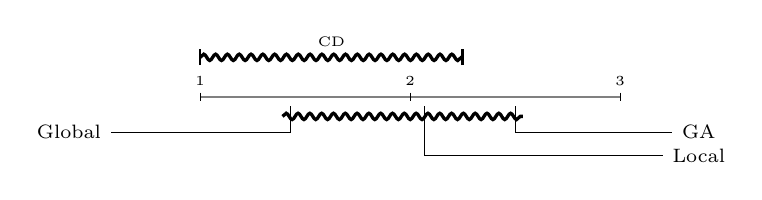
\begin{tikzpicture}[xscale=2]
\node (Label) at  (02.1667,0.7) {\tiny{CD}}; % the label
\draw[decorate,decoration={snake,amplitude=.4mm,segment length=1.5mm,post length=0mm}, very thick, color = black](01.3333, 0.5) -- (03.0000, 0.5);
\foreach \x in {01.3333,03.0000} \draw[thick,color = black] (\x, 0.4) -- (\x, 0.6);

\draw[gray, thick](01.3333, 0) -- (04.0000, 0);
\foreach \x in {01.3333,02.6667,04.0000}\draw (\x cm,1.5pt) -- (\x cm, -1.5pt);
\node (Label) at (01.3333,0.2) {\tiny{1}};
\node (Label) at (02.6667,0.2) {\tiny{2}};
\node (Label) at (04.0000,0.2) {\tiny{3}};
\draw[decorate,decoration={snake,amplitude=.4mm,segment length=1.5mm,post length=0mm}, very thick, color = black](01.8567,-00.2500) -- ( 03.3833,-00.2500);
\node (Point) at (01.9067, 0){};  \node (Label) at (0.5,-00.4500){\scriptsize{Global}}; \draw (Point) |- (Label);
\node (Point) at (03.3333, 0){};  \node (Label) at (4.5,-00.4500){\scriptsize{GA}}; \draw (Point) |- (Label);
\node (Point) at (02.7600, 0){};  \node (Label) at (4.5,-00.7500){\scriptsize{Local}}; \draw (Point) |- (Label);
\end{tikzpicture}
\caption{AUPRC-RF-input.property}
\label{fig:}
\end{figure}
